	\documentclass[10pt,oneside]{CBFT_book}
	% Algunos paquetes
	\usepackage{amssymb}
	\usepackage{amsmath}
	\usepackage{graphicx}
	\usepackage{libertine}
	\usepackage[bold-style=TeX]{unicode-math}
	\usepackage{lipsum}

	\usepackage{natbib}
	\setcitestyle{square}

	\usepackage{polyglossia}
	\setdefaultlanguage{spanish}
	



	\usepackage{CBFT.estilo} % Cargo la hoja de estilo

	% Tipografías
	% \setromanfont[Mapping=tex-text]{Linux Libertine O}
	% \setsansfont[Mapping=tex-text]{DejaVu Sans}
	% \setmonofont[Mapping=tex-text]{DejaVu Sans Mono}

	%===================================================================
	%	DOCUMENTO PROPIAMENTE DICHO
	%===================================================================

\begin{document}

% =================================================================================================
\chapter{Introducción al momento angular (rotaciones)}
% =================================================================================================

El operador $\hat{L}$ será el encargado de realizar las rotaciones. Por el álgebra visto en la mecánica 
clásica sabemos que, dado un vector \vb{v} y una matriz ortogonal $R$ se tiene
\[
	\vb{v}' = R \vb{v} \qquad \text{con} \quad |\vb{v}'|=|\vb{v}|
\]
y 
\[
	|\vb{v}|^2 = V^t V = (V^t R^t) (R V) \qquad \text{pues} \quad R^tR=RR^t = \mathbb{1}
\]
puesto que es una matriz ortogonal. Luego se cumplen 
\[
	clausura	
\]
el producto de dos matrices ortogonales es otra matriz ortogonal
\[
	asociatividad
\]
\[
	E identidad
\]
\[
	E inversa
\]

\subsection{No conmutatividad de las rotaciones clásicas}

Las rotaciones finitas no conmutan. Luego, el grupo de las rotaciones será un grupo abeliano
\[
	R_z(\varphi) = \begin{pmatrix}
	 \\
	\end{pmatrix}
\]
\[
	R_x(\varphi) = \begin{pmatrix}
	 \\
	\end{pmatrix}
\]
\[
	R_y(\varphi) = \begin{pmatrix}
	 \\
	\end{pmatrix}
\]

\begin{figure}[htb]
	\begin{center}
	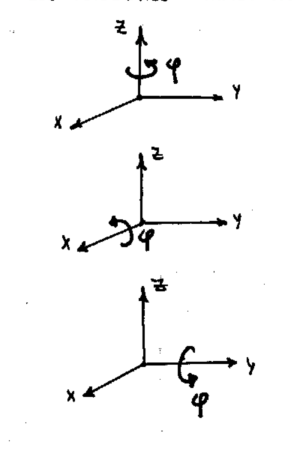
\includegraphics[width=0.6\textwidth]{images/teo2_10.pdf}
	\end{center}
	\caption{}
\end{figure} 

Si reemplazamos $\cos(\epsilon) \approx 1 - \epsilon^2/2$ y $\sin(\epsilon) \approx \epsilon$ hasta orden dos.
Se puede ver que las rotaciones, en torno a ejes diferentes, sólo conmutan a orden uno $(\epsilon)$ de manera 
que una rotación infinitesimal $d\varphi$ conmuta pero una rotación finita $\varphi$ no lo hace.

% =================================================================================================
\section{Rotaciones cuánticas}
% =================================================================================================

Para las rotaciones cuánticas se pedirá
\[
	D,
\]
rotación infinitesimal o bien
\[
	D,
\]
para rotación finita. Donde $\hat{D}$ es el operador de las rotaciones y $\hat{J}$ es un momento angular 
general. Se postula de esta forma para que $\hat{D}$ cumpla las mismas propiedades que $R$ y la relación de 
conmutación
\[
	R_x R_y - R_y R_x = R_z (\epsilon^2) - \mathbb{1}
\]
\[
	D
\]
de modo que la cuenta lleva a  
\[
	J_x
\]
la cual generalizando se llega a 
\[
	[J_i,J_j] = i \hbar \epsilon_{ijk} J_k
\]
que son las relaciones de conmutación generales para momento angular $\hat{J}$.

Para sistemas de spín $1/2$ es 
\[
	D(\hat{n},\phi) \equiv \euler^{-i/\hbar \vb{S}\cdot\hat{n} }
\]
Se puede ver que ante rotaciones cuánticas $D(\hat{n},\phi)$ los valores de expectación transforman como 
vectores
\[
	=
\]

En general $\vb{J} = (J_x, J_y, J_z)$ se transforma como vector y entonces $\hat{J}$ es un operador vectorial.
Para spín $1/2$ es
\[
	\Ket{alpha} =
\]
\[
	D
\]
\[
	D
\]
Si $\phi=2\pi$ (cosa que debiera dejar al ket incólume) se tiene 
\[
	D
\]

Luego, esto es una muestra del carácter no-clásico del spin; una vuelta completa le cambia el signo al ket 
pero notemos cuidadosamente que el valor de expectación -- que es algo físico -- no varía. Esto muestra que 
el ket no puede tener sentido físico.

\subsection{Angulos de Euler}

Se define una serie de rotaciones 
\[
	1 2 3
\]
lo cual equivale a
\[
	R() = 
\]
\[
	\euler
\]

Pero desconozco cómo operar en los ejes móviles $z',y'$
\[
	R_{y'}(\beta) =
\]
\[
	R_{z'}(\gamma) =
\]
\[
	R() =
\]
Rotación equivalente a [1] pero para ejes fijos, puesto que en mecánica cuántica sabemos rotar en torno a 
ejes fijos.

Los ángulos de Euler son la caracterización de una rotación general en 3D.

Entonces nuestra rotación en 3D cuántica será:
\[
	D() =
\]

\subsection{Autoestados y autovalores de J}

Partimos de 
\[
	[] = 
\]
y
\[
	J^2 = , [J^2,J] = 0
\]
siendo la última muy importante y probándose por evaluación directa. Lleva a 
\[
	[J^2,J_i^n] = 0 \qquad \text{con} \; i=x,y,z \; n\in\mathbb{N}
\]

Se eligen $J^2, J_z$ como observables que conmutan 
\[
	J^2
\]

Definiremos los operadores de subida y de bajada
\[
	J_{\pm} \equiv J_x \pm J_y
\]
que verifican 
\[
	[]
\]
Entonces se tiene 
\[
	J^2() \longrightarrow 
\]
\[
	(J_z) \longrightarrow
\]

\[
	J_{\pm} \Ket{a,b} = C_{\pm} \Ket{a,b\pm\hbar}
\]
\[
	J_+
\]
sube el $J_z$ en una unidad de $\hbar$ o bien baja el $J_z$ en una unidad de $\hbar$.
\[
	J_+J_- =  ,
\]
\[
	J^2 = ,  
\]
\[
	\Braket{a,b|J^2 - J^2_z|a,b} = 
\]
\[
	(a-b^2)\Braket{a,b|a,b} = , a \geq b^2
\]
hay cota para $b$.
Como no puede seguir subiendo debe dar el ket nulo 
\[
	= 0
\]
\[
	= 0
\]
pero 
\[
	J_-J_+
\]
\[
	= 0	\qquad a = b_m(b_m-\hbar)
\]
tiene solución 
\[
	b_M - B_m = - \hbar
\]
pero esto es absurdo.

Luego,
\[
	\Ket{a,b_m} \longrightarrow \Ket{a,b_M}
\]
y como $J_+$ sube de a un $\hbar$ será
\[
	b_M = b_m + n\hbar
\]
y entonces
\[
	b_M = \frac{n\hbar}{2} = \frac{n}{2} \hbar = j \hbar
\]
y se da que $j$ es entero o semientero.

Definiremos 
\[
	b_M \equiv j \hbar \qquad a \equiv j (j+1) \hbar^2 \qquad -j\hbar \leq b \leq j\hbar
\]
pero como $b/\hbar = m$
\[
	b_M \equiv j \hbar \qquad a \equiv j (j+1) \hbar^2 \qquad -j \leq m \leq j
\]
\[
	m = (-j,-j+1,-j+2,...,j-1,j) \qquad 2j+1 \text{valores de} \; m
\]
\[
	J^2 \Ket{j,m} = j( j+1 )\hbar^2\Ket{j,m} \qquad J_z \Ket{j,m} = m \hbar \Ket{j,m}
\]

\subsection{La normalización de $J_\pm$}

\[
	J_+
\]
\[
	\Braket{j,m|J_-J_+|j,m} = 
\]
\[
	c_+ = 
\]
\[
	\Braket{j,m|J_+J_-|j,m} = 
\]
\[
	c_- =
\]
\[
	J_+
\]

\subsection{Elementos de matriz de $J^2, J_z, J_+$}

Asumiendo normalización de $\Ket{j,m}$ se tiene 
\[
	\Braket{} = 
\]
\[
	=
\]

\subsection{Elementos de matriz de $\mathcal{D}(R)$}

Ahora queremos ver cual es la forma de los elementos de matriz de $\mathcal{D}(R)$
\[
	\mathcal{D}(R) =
\]
siendo que $\mathcal{D}(R)$ tiene por efecto rotar el sistema físico.
Lo primero que hay que notar es que 
\[
	\propto \delta_{jj'}
\]
porque $[J^2,J_i]=0$ y entonces $[J^2,J_i^n]=0$ y 
\[
	D
\]
y 
\[
	D
\]
es una matriz para cada $j$ fijo con $\{ (2j+1)\times(2j+1)=\text{dimensión}\}$
\[
	D
\]
pero las rotaciones no cambian el $j$, $\mathcal{D}(R)$ conecta estados con la misma $j$ y $\mathcal{D}(R) 
\in (2j+1)\times(2j+1)$ 
\[
	D
\]

La matriz de $\mathcal{D}(R)$ (no caracterizada por un único $j$) puede ponerse en forma diagonal por bloques:


con cada bloque de $(2j+1)\times(2j+1)$ , pero siendo cada bloque irreducible. Las matrices de rotación con 
$j$ fijo forman un grupo. $\mathcal{D}_{m'm}^{(j)}(R)$ son los elementillos de la matriz.
\[
	\Ket{j,m} \longrightarrow
\]

\subsection{Forma explícita del operador $\mathcal{D}(R)$}

Los ángulos de Euler permitieron caracterizar la rotación más general. Entonces 
\[
	D
\]
\[
	D
\]

En los $d_{m'm}^{(j)}$ está la dificultad de la cuenta.

% =================================================================================================
\section{Formalismo de spinores de Pauli}
% =================================================================================================

Apropiado para trabajar con sistemas de spín $1/2$. Estos sistemas son casos particulares de momento angular,
\[
	j = 1/2 \qquad m=-\frac{1}{2},+\frac{1}{2}
\]
y se definen los spinores $\chi_\pm$ como
\[
	\Ket{+} \equiv  \begin{pmatrix}
	                 1 \\ 0 
	                \end{pmatrix} \equiv  \chi_+
\]

Para spín $1/2$ podemos tomar $\vb{J} = \vb{S}$ por la analogía de las relaciones de conmutación.
A su vez 
\[
	\vb{S} = \frac{\hbar}{2} \vec{\sigma} \; \text{con} \;
\]
que es una especie de vector 
\[
	\sigma
\]
Luego esta equivalencia provee expresión de los operadores $S_i$ en términos de matrices de $2\times 2$, así:
\[
	\frac{i}{2}[ J_- - J_+] = J_y = S_y = \frac{\hbar}{2} \sigma_y
\]

Las matrices de Pauli cumplen las propiedades básicas siguientes 
\[
	\sigma^2_i = \mathbb{1}
\]
\[
	\Ket{+} \qquad (\sigma\dot\vb{a})
\]

\subsection{Aplicación a las rotaciones}

\[
	D
\]
pero 
\[
	()^n= 
\]
\[
	\euler
\]
\[
	d
\]
es el operador de rotación para sistemas de spin $1/2$. Con esta expresión podemos evaluar 
$d^{j=1/2}_{m'm}(\beta)$
\[
	d
\]
donde hemos usado los resultados 
\[
	\cos \sin 
\]

En el caso general el operador de rotación para sistemas de spin $1/2$ lucirá:
\[
	D = 
\]

\subsection{Ejemplo}

\[
	d
\]
Este resultado es intuitivamente lógico.


\subsection{Rotaciones en sistemas con $j=1$}

Ahora tenemos 
\[
	j=1 \qquad m = -1,0,1
\]
recordando $J_y$ en términos de escaleras
\[
	J_y
\]
\[
	\euler
\]
\[
	\left( \frac{J_y}{\hbar} \right)^n =
\]
\[
	\euler =
\]
acá lo vemos como operador (es notación), $d_{m'm}^{j=1}(\beta)$ simboliza la matriz
\[
	d
\]

% =================================================================================================
\section{Momento angular orbital}
% =================================================================================================

\[
	\vb{L} =
\]
verifica el álgebra de $\vb{J}$,
\[
	[]
\]
Consideremos ahora una rotación en torno a $z$, en un $\delta\phi$,
\[
	() =
\]
\[
	() = 
\]
esto es una traslación en $\hat{x},\hat{y}$,
\[
	(1-i\frac{L_z}{\hbar}\delta\phi) \Ket{x',y',z'} = \Ket{}
\]

Esta traslación es debida a una rotación infinitesimal en $\delta\phi$ torno a $z$ entonces genera las 
rotaciones clásicas en torno a $z$.
\[
	\Psi 
\]
\[
	\Psi
\]

Podemos hallar una expresión para $L_z$ en esféricas:
\[
	\Braket{r,\theta,\varphi||\alpha}
\]
identificamos 
\[
	= 
\]
operador $L_z$ en esféricas

Usando 
\[
	L^2 = 
\]
\[
	\Braket{L^2}
\]
\[
	L^2 = -\hbar^2 r^2 \nabla^2_{\theta,\varphi}
\]
donde $\nabla^2_{\theta,\varphi}$ es la parte angular del laplaciano en coordenadas esféricas.
Esto puede obtenerse también partiendo de 
\[
	L^2 = \vb{x}^2\vb{p}^2 - (\vb{x}\cdot\vb{p})^2 + i\hbar \vb{x}\cdot\vb{p}
\]

Sea un $H$ de partícula, sin spín, sujeta a potencial simétricamente esférico. Sabemos que la función de onda 
$\Psi_\alpha(\vb{r}')$ es separable en coordenadas esféricas, entonces:
\[
	\Braket{|} = 
\]
\[
	\Braket{|} = 
\]

Cuando el H es esféricamente simétrico (como en un potencial central) se tiene 
\[
	[] = [] = 0
\]

Trabajaremos solamente en la parte angular  $\Ket{\theta,\varphi} \equiv \Ket{\hat{n}}$
\[
	\Braket{\hat{n}|\ell,m} =
\]
que es la amplitud de hallar $\Ket{\ell,m}$ en la dirección $\hat{n}$.

Podemos vincular ahora los armónicos esféricos con los autoestados de $L_z,L^2$
\[
	L_z
\]
\[
	L^2
\]
\[
	=
\]
Entonces, con la ortogonalidad
\[
	\longrightarrow
\]
y con la completitud 
\[
	\longrightarrow
\]
de manera que llegamos a 
\[
	\int \int 
\]

Podemos hallar una expresión para 
\[
	= 0
\]
\[
	\Rightarrow
\]

Luego usamos $L_-$ para hallar sucesivamente los demás $Y^m_\ell$
\[
	=
\]
y por este camino se llega a 
\[
	Y
\]
con 
\[
	\qquad 
\]

En el caso de momento angular orbital $\ell$ no puede ser semientero porque entonces $m$ sería semientero y 
en una vuelta de $2\pi$
\[
	\euler^{im2\pi} = -1
\]	

Además,
\[
	\text{(no hay signo menos)}
\]


% \bibliographystyle{CBFT-apa-good}	% (uses file "apa-good.bst")
% \bibliography{CBFT.Referencias} % La base de datos bibliográfica

\end{document}
